% Template: LLNCS (Springer Lecture Notes in Computer Science)
% ITP has used LLNCS in multiple years. If the CFP specifies LIPIcs,
% change \documentclass to lipics and adjust the preamble accordingly.
\documentclass[runningheads]{llncs}

\usepackage[T1]{fontenc}
\usepackage{graphicx}
\usepackage{booktabs}
\usepackage{amsmath,amssymb}
\usepackage{hyperref}
\usepackage{xcolor}
\usepackage{multirow}
\usepackage{array}

\hypersetup{
  colorlinks=true,
  linkcolor=blue,
  citecolor=blue,
  urlcolor=blue
}

\newcommand{\enquote}[1]{``#1''}

\begin{document}

\title{Provenance-Conditional Hyperbolic Graph Learning\\on Traced Formal-Math Hierarchies:\\Pipeline, Protocol, Diagnostics, and Evidence Boundaries}

\author{Anonymous Author(s)}
\institute{Anonymous Institution}
\maketitle

\begin{abstract}
We present a reproducible pipeline, evaluation protocol, diagnostics framework, training alignment correction, and an ancestor explanation tool for studying graph representation learning on real traced Lean/Mathlib hierarchy graphs.
Our central finding is provenance-conditional: on the full source graph (containing both \texttt{extends} and \texttt{instance\_of} edges), GCN remains stronger; HGCN's advantage emerges only on the explicit hierarchy layer (\texttt{extends} edges alone), where genuine depth exists, and grows monotonically with ancestor chain depth (+0.03 at hop\_2 to +0.27 at hop\_4\_plus).

Contributions: (C1) a version-locked extraction pipeline from traced repositories to relation-aware subgraphs; (C2) a grouped multi-positive ancestor retrieval protocol with query-level splits and hop-bucket analysis; (C3) a structural diagnostics framework with heuristic classification thresholds; (C4) the first demonstration that edge provenance composition---not graph size or capacity---determines which geometry is favored; (C5) migration from binary edge classification to query-grouped retrieval training.
We validate through 60 provenance-aware seed sweeps (zero failures) across two candidate graphs and three provenance splits, and demonstrate downstream proof-engineering relevance via an ancestor explanation tool.

Evidence is from reviewed single-environment runs; the finding is established on two candidate graphs (133 and 253 nodes).
\end{abstract}

\section{Introduction}

\subsection{Motivation}

Interactive theorem provers such as Lean, Coq, and Isabelle organize mathematical knowledge in rich hierarchical structures. In Lean/Mathlib, declarations (definitions, theorems, type classes) are connected by \texttt{extends} edges (explicit inheritance), \texttt{instance\_of} edges (synthesized type-class instance registrations), and \texttt{uses} edges (referential dependencies). These hierarchy graphs are natural targets for graph representation learning: the hierarchical structure encodes mathematical knowledge at multiple levels of abstraction, and navigating this hierarchy efficiently could support proof search, declaration recommendation, and mathematical knowledge exploration.

Hyperbolic graph neural networks (HGCN) offer a theoretically appealing inductive bias for such data: hyperbolic space can embed tree-like structures with exponentially lower distortion than Euclidean space, and the distance scaling properties of hyperbolic geometry are well-suited to representing ancestor--descendant relationships. However, empirical evidence for hyperbolic advantage on real formal-math graphs has been mixed. Prior work has reported that HGCN does not consistently outperform Euclidean baselines (GCN) on traced Lean hierarchy graphs, raising the question: under what structural conditions does the hyperbolic inductive bias actually help?

\subsection{Background}

\textbf{Lean/Mathlib hierarchy semantics.}
Lean 4 and its mathematical library Mathlib organize knowledge through a type-class hierarchy. Declarations (definitions, theorems, instances) are connected by two primary hierarchy edge types: \texttt{extends} edges encode explicit inheritance (e.g., \texttt{CommRing} extends \texttt{Ring} extends \texttt{Semiring}), creating chains of increasing abstraction with genuine depth and branching; \texttt{instance\_of} edges register synthesized type-class instances (e.g., \texttt{Int.instCommRing} is an instance of \texttt{CommRing}), connecting concrete implementations to abstract interfaces without creating inheritance chains. A third edge type, \texttt{uses}, captures referential dependencies but does not participate in the hierarchy layer. This distinction between explicit and synthesized hierarchy edges is Lean-specific and has not been systematically controlled for in prior graph-learning experiments on formal-math data.

\textbf{Hyperbolic graph neural networks.}
Hyperbolic space offers exponentially lower distortion for embedding tree-like structures compared to Euclidean space. HGCN (Hyperbolic Graph Convolutional Networks) leverages this by performing message passing in hyperbolic geometry, with a learnable curvature parameter. The theoretical motivation is that ancestor--descendant relationships in hierarchies should be more naturally captured by hyperbolic distance scaling. However, the practical benefit depends on the actual tree-likeness of the input graph: on flat or shallow structures, the additional representational capacity of hyperbolic geometry can be a liability rather than an advantage.

\textbf{Formal-math graph tooling.}
Prior work on graph-based approaches to formal mathematics has focused on premise retrieval, proof search guidance, and declaration recommendation. These efforts typically treat the graph as a uniform structure without distinguishing edge provenance. Our work differs in focus: rather than proposing a new model architecture, we provide the methodological infrastructure---pipeline, protocol, diagnostics---needed to systematically determine \emph{under which structural conditions} different representation geometries are effective.

\subsection{The Problem}

We identify two categories of confounds that have obscured the answer to this question:

\textbf{Protocol confounds.}
The standard evaluation protocol for ancestor retrieval in formal-math graphs has historically treated the task as single-positive ranking---finding one true ancestor among candidates. In reality, the task is multi-positive: a given \texttt{(declaration, relation)} query has multiple true ancestors at varying hop distances. The legacy protocol also used edge-level random splits, which can fragment the same query's positive set across train/val/test, and binary edge classification training (BCEWithLogitsLoss), which optimizes per-edge existence rather than within-query ranking quality.

\textbf{Structural confounds.}
Real traced Lean/Mathlib hierarchy graphs are not uniform trees. The relation layer is often shallow and fragmented, with a high proportion of \texttt{instance\_of} edges that are structurally flat---they register type-class instances without creating inheritance chains. Mixing these flat synthesized edges with genuine \texttt{extends} hierarchy edges may dilute the hierarchical signal that hyperbolic geometry is designed to exploit, but this composition effect has not been systematically controlled for.

\subsection{Our Approach}

We address these confounds through a staged experimental pipeline:

\begin{enumerate}
\item \textbf{Pipeline and protocol freeze} (Milestone 1): Version-lock the entire data-processing chain and freeze a grouped multi-positive ancestor retrieval protocol with query-level splits and hop-bucket analysis.
\item \textbf{Diagnostics and candidate selection} (Milestone 2): Characterize the structural properties of real formal-math graphs (longest chain, leaf ratio, component structure, multi-parent branching, cycle rank, delta-hyperbolicity proxy) and select candidates that span the range from shallow star forests to deeper hierarchies.
\item \textbf{Training alignment} (Milestone 3): Migrate from binary edge classification to query-grouped retrieval training (sampled softmax / InfoNCE-family loss), align training query keys to evaluation query keys \texttt{(src\_id, relation\_type)}, and establish matched GCN/HGCN baselines on the full source graph.
\item \textbf{Provenance split} (Milestone 4): Systematically decompose the source graph into three provenance layers---\texttt{explicit\_only} (extends edges alone), \texttt{synthesized\_only} (instance\_of edges alone), and \texttt{hierarchy\_mixed} (both)---and repeat the matched comparison on each layer.
\item \textbf{Proof-side bridge} (Milestone 5): Demonstrate that the provenance-conditional finding has concrete implications for proof-engineering tool quality via an ancestor explanation CLI tool.
\end{enumerate}

\subsection{Central Claim}

\textbf{Edge provenance composition is a first-class experimental variable in formal-math hierarchy graph learning.} On real traced Lean/Mathlib graphs, HGCN outperforms GCN only when the graph is restricted to explicit (\texttt{extends}) hierarchy edges; adding synthesized (\texttt{instance\_of}) edges---which are structurally flat---dilutes the hierarchical signal enough to revert the comparison in GCN's favor.

\subsection{Non-Claims (Explicit Boundaries)}

\begin{enumerate}
\item We do \textbf{not} claim that HGCN is generally superior to GCN on formal-math graphs.
\item We do \textbf{not} claim that the provenance-conditional finding generalizes beyond the two reviewed candidate graphs (Field.Subfield: 133 nodes, Order.Ring: 253 nodes).
\item We do \textbf{not} claim clean-room reproducibility has been fully closed; current evidence comes from reviewed single-environment runs.
\item We do \textbf{not} claim the pipeline covers full Mathlib or end-to-end theorem proving.
\item We do \textbf{not} claim the diagnostics thresholds are theoretically optimal; they are empirically calibrated heuristics from reviewed artifacts.
\end{enumerate}

\subsection{Contributions Summary}

\begin{itemize}
\item \textbf{C1.} Reproducible traced formal-math hierarchy graph pipeline: version-locked from Lean/Mathlib traced repositories through declaration graphs, precise hierarchy extraction, coverage-aware repair, and relation-aware subgraph construction.
\item \textbf{C2.} Grouped multi-positive ancestor retrieval protocol: standardized evaluation with query-level split disjointness, MAP/nDCG/nDCG@10/MRR/Recall@k metrics, and hop-bucket analysis.
\item \textbf{C3.} Graph structure diagnostics framework: heuristic thresholds for classifying formal-math graphs as shallow forest, star forest, or hierarchy-rich.
\item \textbf{C4.} Provenance-conditional hyperbolic advantage finding: edge provenance composition---not graph size or model capacity---determines whether hyperbolic geometry helps.
\item \textbf{C5.} Training task alignment correction: migration from binary edge classification to query-grouped retrieval training with aligned query keys.
\end{itemize}

\section{Experimental Setup}

\subsection{Data: Traced Lean/Mathlib Hierarchy Graphs}

Our pipeline extracts hierarchy graphs from traced Lean/Mathlib repositories. The processing chain consists of:
\begin{enumerate}
\item \textbf{Tracing}: Running LeanDojo on target repositories to produce normalized traces.
\item \textbf{Declaration graph construction}: Extracting nodes (declarations) and edges (extends, instance\_of, uses) from trace data.
\item \textbf{Precise hierarchy extraction}: Filtering to \texttt{extends} and \texttt{instance\_of} edges that form the hierarchy layer.
\item \textbf{Coverage-aware repair}: Handling unresolved endpoints---endpoints that can be backfilled are repaired; those that cannot are explicitly annotated and excluded from negative sampling.
\item \textbf{Relation-aware subgraph construction}: Extracting subgraphs centered on specific Mathlib modules (e.g., \texttt{Mathlib.Algebra.Field.Subfield}, \texttt{Mathlib.Algebra.Order.Ring}).
\end{enumerate}

\textbf{Candidate graphs.}
We select two candidate graphs for formal evaluation:

\begin{table}[h]
\centering
\caption{Candidate graphs for formal evaluation.}
\label{tab:candidates}
\begin{tabular}{llrrl}
\toprule
Graph & Source Module & Nodes & Edges & Relations \\
\midrule
Field.Subfield & \texttt{Mathlib.Algebra.Field.Subfield} & 133 & 152 & extends, instance\_of \\
Order.Ring & \texttt{Mathlib.Algebra.Order.Ring} & 253 & 300 & extends, instance\_of \\
\bottomrule
\end{tabular}
\end{table}

These candidates were selected through the diagnostics framework (C3) to represent a range from a smaller, more controlled probe (Field.Subfield) to a larger, more balanced candidate (Order.Ring). Both contain only \texttt{extends} and \texttt{instance\_of} edges (no \texttt{uses} edges in the hierarchy layer).

\subsection{Provenance Split Design}

We decompose each source graph into three provenance layers based on the origin of each edge:

\begin{table}[h]
\centering
\caption{Provenance split design.}
\label{tab:provenance-split}
\begin{tabular}{lll}
\toprule
Split & Edges Included & Structural Role \\
\midrule
\texttt{explicit\_only} & \texttt{extends} only & \textbf{Primary evidence}: isolates genuine hierarchy \\
\texttt{synthesized\_only} & \texttt{instance\_of} only & \textbf{Controlled diagnostic}: confirms flat structure \\
\texttt{hierarchy\_mixed} & Both & \textbf{Reproducibility check}: full source graph \\
\bottomrule
\end{tabular}
\end{table}

The provenance split protocol is frozen with origin mapping: \texttt{extends}~$\to$~explicit, \texttt{instance\_of}~$\to$~synthesized, both~$\to$~\texttt{hierarchy\_mixed}. The \texttt{hierarchy\_mixed}~=~full source graph identity has been programmatically verified for both candidates.

\subsection{Structural Properties by Provenance Split}

The provenance split produces dramatically different structural profiles (Figure~\ref{fig:provenance-structure}):

\begin{table}[h]
\centering
\caption{Structural properties of candidate graphs by provenance split. \texttt{synthesized\_only} graphs are flat star forests (longest chain = 1, multi-parent = 0, cycle rank = 0). All hierarchy depth comes from \texttt{explicit\_only} edges.}
\label{tab:structural}
\begin{tabular}{lrrrrrr}
\toprule
Property & \multicolumn{3}{c}{Field.Subfield} & \multicolumn{3}{c}{Order.Ring} \\
\cmidrule(lr){2-4} \cmidrule(lr){5-7}
& explicit & synth. & mixed & explicit & synth. & mixed \\
\midrule
Longest chain    & 9  & 1  & 10  & 10  & 1  & 10  \\
Multi-parent     & 40 & 0  & 40  & 66  & 0  & 66  \\
Cycle rank       & 32 & 0  & 32  & 60  & 0  & 60  \\
Leaf ratio       & 0.124 & 0.537 & 0.278 & 0.208 & 0.656 & 0.502 \\
$\delta$/maxdist & 0.286 & 0.000 & --- & 0.136 & 0.000 & --- \\
Giant comp.\ ratio & 0.506 & --- & --- & 0.792 & --- & --- \\
\bottomrule
\end{tabular}
\end{table}

\begin{figure}[t]
\centering
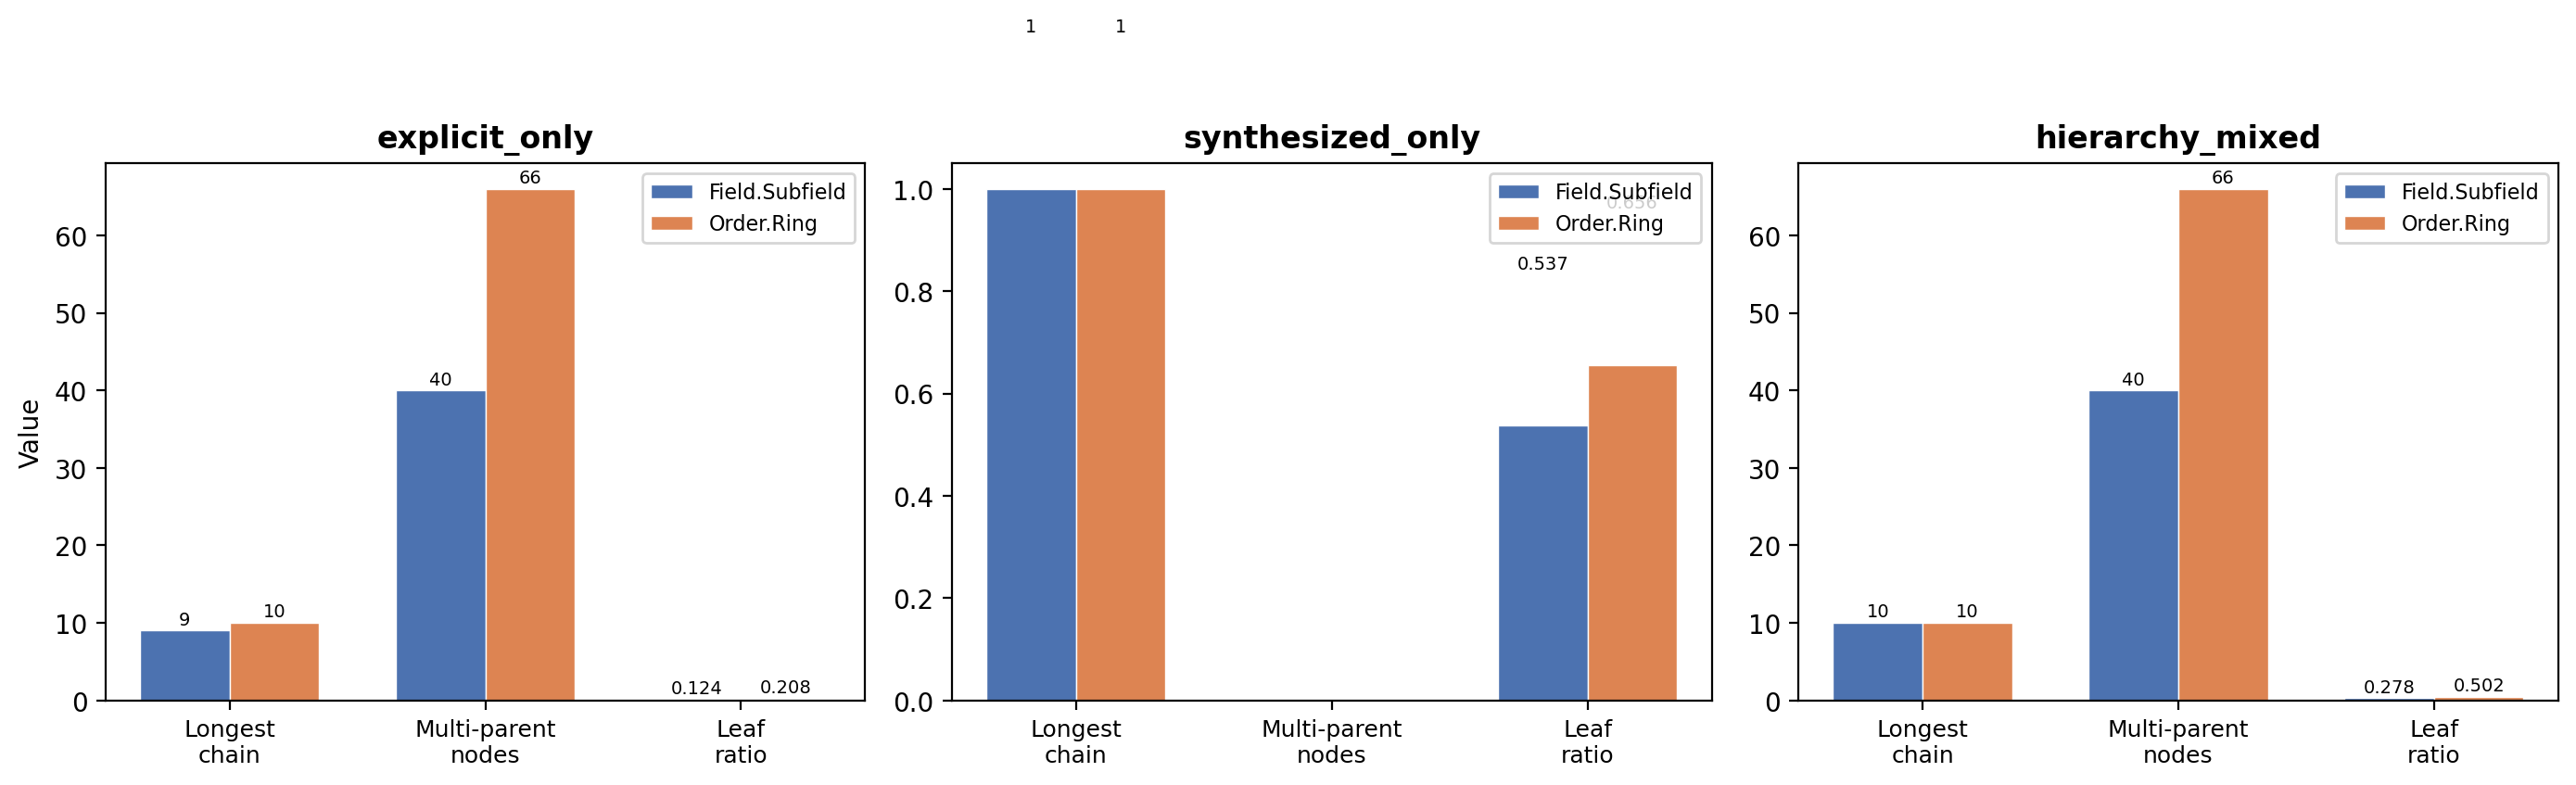
\includegraphics[width=\textwidth]{figures/F1_provenance_structure.png}
\caption{Structural contrast across provenance splits. Left: \texttt{explicit\_only} graphs exhibit genuine hierarchy depth (longest chain 9--10, multi-parent 40--66). Right: \texttt{synthesized\_only} graphs are flat star forests (longest chain 1, multi-parent 0). Center: \texttt{hierarchy\_mixed} inherits depth from explicit edges but gains leaf inflation from synthesized edges.}
\label{fig:provenance-structure}
\end{figure}

Key observation: \texttt{synthesized\_only} graphs are shallow star forests (longest chain = 1, multi-parent = 0, cycle rank = 0). All hierarchy depth comes from \texttt{explicit\_only} edges. Adding synthesized edges to form \texttt{hierarchy\_mixed} does not add meaningful depth---it inflates leaf ratio and fragmentation without contributing to hierarchy structure.

\subsection{Evaluation Protocol}

We use the \textbf{grouped multi-positive ancestor retrieval} protocol (C2):
\begin{itemize}
\item \textbf{Query}: \texttt{(src\_id, relation\_type)}---a declaration and a relation type.
\item \textbf{Positives}: All true ancestors of \texttt{src\_id} reachable via \texttt{extends} edges for the given relation type.
\item \textbf{Split}: Query-level disjoint---all positives for the same \texttt{(src, relation)} query remain in the same split. Split ratios: val\_ratio = 0.15, test\_ratio = 0.15.
\item \textbf{Metrics}: MAP, nDCG, nDCG@10, MRR, Recall@k.
\item \textbf{Hop-bucket analysis}: Results decomposed by ancestor distance: hop\_2, hop\_3, hop\_4\_plus.
\end{itemize}

This protocol replaces the legacy single-positive \texttt{ancestor\_ranking} approach, which treated ancestor retrieval as finding one positive among candidates, ignoring the multi-positive nature of the task.

\subsection{Models and Training}

We compare two models under matched conditions:

\textbf{GCN (Euclidean baseline):} Standard graph convolutional network operating in Euclidean space.

\textbf{HGCN (Hyperbolic):} Hyperbolic graph convolutional network with curvature parameter, residual connections, and distance signal integration (variant: \texttt{relation\_hgcn\_residual\_v3}).

\textbf{Matched training configuration:}

\begin{table}[h]
\centering
\caption{Matched training configuration for all experiments.}
\label{tab:config}
\begin{tabular}{ll}
\toprule
Parameter & Value \\
\midrule
Dimensions (input/hidden/output) & 16 / 16 / 16 \\
Grouped loss & sampled\_softmax \\
Negative ratio & 10.0 \\
Optimizer & SGD, lr = 0.01 \\
Weight decay & 1e-4 \\
Epochs & 100 \\
Eval every & 5 epochs \\
Patience & 12 \\
Seeds & [7, 42, 123, 2026, 3407] \\
\bottomrule
\end{tabular}
\end{table}

Training uses query-grouped retrieval loss (C5) with query keys \texttt{(src\_id, relation\_type)} aligned to the evaluation protocol. Model selection uses validation grouped MAP.

\subsection{Experimental Design}

The experimental design consists of three phases:

\begin{enumerate}
\item \textbf{Milestone 3 baseline} (T32/T33): Matched GCN vs HGCN grouped 5-seed sweeps on \texttt{hierarchy\_mixed} (full source graph). 20 runs (2 models $\times$ 2 graphs $\times$ 5 seeds, zero failures).
\item \textbf{Provenance-aware sweeps} (T42): Matched GCN vs HGCN grouped 5-seed sweeps on all three provenance splits. 60 runs total (2 models $\times$ 2 graphs $\times$ 3 splits $\times$ 5 seeds, zero failures).
\item \textbf{Proof-side bridge} (T52a): Ancestor explanation CLI tool that loads T42 reviewed node embeddings and performs provenance-aware ancestor retrieval ranking.
\end{enumerate}

\section{Results}

\subsection{Milestone 3 Baseline: Full Source Graph (hierarchy\_mixed)}

On the full source graph (equivalent to \texttt{hierarchy\_mixed}), GCN outperforms HGCN on both candidates:

\begin{table}[h]
\centering
\caption{Grouped retrieval results on \texttt{hierarchy\_mixed} (full source graph). GCN vs HGCN, 5-seed mean $\pm$ std.}
\label{tab:baseline}
\begin{tabular}{lrrrrr}
\toprule
Graph & GCN MAP & HGCN MAP & Delta & GCN nDCG & HGCN nDCG \\
\midrule
Field.Subfield & $0.4839 \pm 0.0783$ & $0.4458 \pm 0.1150$ & GCN +0.0381 & $0.6428 \pm 0.0653$ & $0.6095 \pm 0.0908$ \\
Order.Ring     & $0.5789 \pm 0.0346$ & $0.5616 \pm 0.0312$ & GCN +0.0173 & $0.7293 \pm 0.0340$ & $0.7111 \pm 0.0296$ \\
\bottomrule
\end{tabular}
\end{table}

\textbf{Interpretation}: Under the matched grouped protocol on the full source graph, GCN remains the stronger model. This is consistent with the original observation that hyperbolic inductive bias does not confer a general advantage on these graphs. However, this baseline does not control for edge provenance composition---the full graph mixes genuine hierarchy edges with flat synthesized edges.

\subsection{Primary Evidence: explicit\_only}

On \texttt{explicit\_only} graphs---which isolate genuine hierarchy structure---HGCN outperforms GCN on both candidates across all primary ranking metrics:

\begin{table}[h]
\centering
\caption{Provenance-aware grouped retrieval results on \texttt{explicit\_only} (primary evidence). 5-seed mean $\pm$ std.}
\label{tab:explicit}
\begin{tabular}{llrrr}
\toprule
Graph & Metric & GCN & HGCN & Delta \\
\midrule
\multirow{4}{*}{Field.Subfield}
& MAP     & $0.5256 \pm 0.0800$ & $0.6503 \pm 0.0481$ & \textbf{+0.1247} \\
& nDCG    & $0.6864 \pm 0.0691$ & $0.7696 \pm 0.0435$ & \textbf{+0.0832} \\
& nDCG@10 & $0.6002 \pm 0.0888$ & $0.6997 \pm 0.0539$ & \textbf{+0.0995} \\
& MRR     & $0.5449 \pm 0.1027$ & $0.6738 \pm 0.0588$ & \textbf{+0.1289} \\
\midrule
\multirow{4}{*}{Order.Ring}
& MAP     & $0.5836 \pm 0.0978$ & $0.6393 \pm 0.0656$ & \textbf{+0.0557} \\
& nDCG    & $0.7332 \pm 0.0725$ & $0.7743 \pm 0.0565$ & \textbf{+0.0411} \\
& nDCG@10 & $0.6224 \pm 0.1347$ & $0.7064 \pm 0.0774$ & \textbf{+0.0840} \\
& MRR     & $0.5888 \pm 0.1472$ & $0.7211 \pm 0.0902$ & \textbf{+0.1323} \\
\bottomrule
\end{tabular}
\end{table}

The Field.Subfield MAP improvement of +0.1247 is the largest model gap observed in the entire project. HGCN outperforms GCN on both candidates across all primary ranking metrics (MAP, nDCG, nDCG@10, MRR).

\subsection{Hop-Bucket Analysis: Advantage Scales with Depth}

HGCN's advantage on \texttt{explicit\_only} grows monotonically with hop depth on both candidates (Figure~\ref{fig:hop-delta}):

\begin{table}[h]
\centering
\caption{Hop-bucket MAP comparison on \texttt{explicit\_only}. HGCN advantage grows monotonically with ancestor chain depth. 5-seed mean $\pm$ std. FS hop\_4\_plus based on 4/5 seeds (seed 2026 produces no hop\_4\_plus queries; symmetric between GCN and HGCN).}
\label{tab:hop-bucket}
\begin{tabular}{llrrr}
\toprule
Graph & Bucket & GCN MAP & HGCN MAP & Delta \\
\midrule
\multirow{3}{*}{Field.Subfield}
& hop\_2      & $0.3403 \pm 0.1295$ & $0.3946 \pm 0.1402$ & +0.0543 \\
& hop\_3      & $0.2321 \pm 0.1402$ & $0.4050 \pm 0.2321$ & \textbf{+0.1729} \\
& hop\_4\_plus$^\dagger$ & $0.2774 \pm 0.1002$ & $0.5245 \pm 0.1419$ & \textbf{+0.2471} \\
\midrule
\multirow{3}{*}{Order.Ring}
& hop\_2      & $0.2347 \pm 0.0352$ & $0.2615 \pm 0.1066$ & +0.0268 \\
& hop\_3      & $0.2038 \pm 0.0486$ & $0.2989 \pm 0.0958$ & \textbf{+0.0951} \\
& hop\_4\_plus & $0.4506 \pm 0.1582$ & $0.7214 \pm 0.0264$ & \textbf{+0.2708} \\
\bottomrule
\end{tabular}
\end{table}

\begin{figure}[t]
\centering
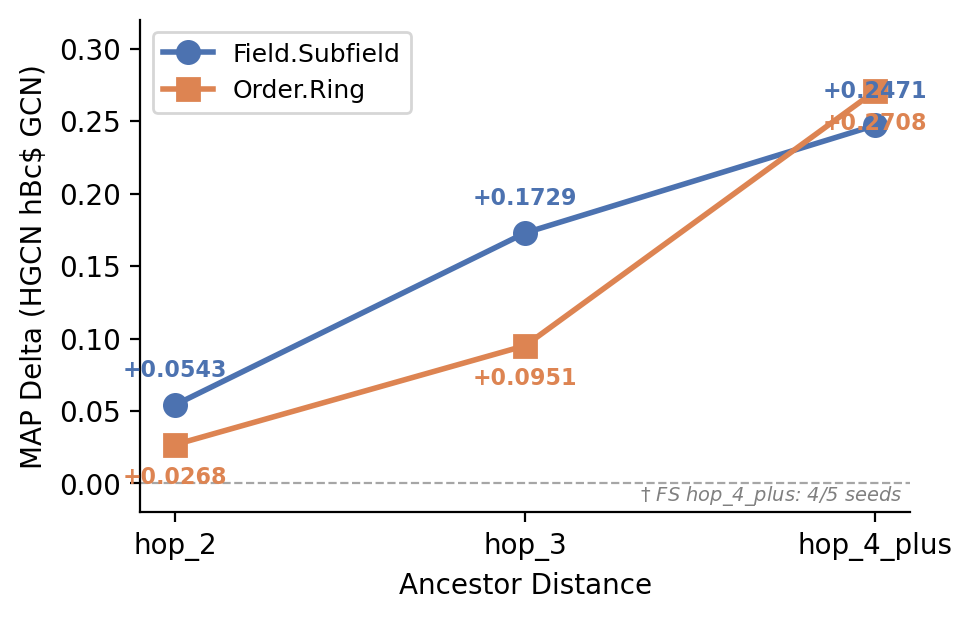
\includegraphics[width=0.6\textwidth]{figures/F2_hop_depth_delta.png}
\caption{HGCN vs GCN MAP delta on \texttt{explicit\_only}, decomposed by hop depth. HGCN's advantage grows monotonically from hop\_2 to hop\_4\_plus on both candidate graphs, confirming that hyperbolic geometry specifically benefits longer ancestor chains.}
\label{fig:hop-delta}
\end{figure}

The HGCN advantage scales from approximately +0.03--0.05 at hop\_2 to approximately +0.25--0.27 at hop\_4\_plus. This monotonic growth is consistent with the theoretical motivation for hyperbolic geometry: the benefit comes from hyperbolic space's ability to embed longer hierarchical paths with lower distortion, not from model capacity.

\subsection{Controlled Diagnostic: synthesized\_only}

On \texttt{synthesized\_only} graphs---which are structurally flat star forests---GCN matches or outperforms HGCN:

\begin{table}[h]
\centering
\caption{Provenance-aware results on \texttt{synthesized\_only} (controlled diagnostic).}
\label{tab:synthesized}
\begin{tabular}{lrrr}
\toprule
Candidate & GCN MAP & HGCN MAP & Delta \\
\midrule
Field.Subfield & $1.0000 \pm 0.0000$ & $0.6857 \pm 0.1140$ & GCN +0.3143 \\
Order.Ring     & $0.8453 \pm 0.0295$ & $0.7560 \pm 0.0761$ & GCN +0.0893 \\
\bottomrule
\end{tabular}
\end{table}

\noindent\textit{Note.} Field.Subfield \texttt{synthesized\_only} is a flat star forest (longest chain = 1, multi-parent = 0); GCN trivially achieves perfect MAP.

\smallskip

GCN matches or outperforms HGCN on the flat synthesized graphs. The hyperbolic inductive bias is a liability on structures with no hierarchy depth, confirming that HGCN's advantage on \texttt{explicit\_only} is driven by geometry matching the graph structure, not by model capacity.

\subsection{Reproducibility Check: hierarchy\_mixed}

The \texttt{hierarchy\_mixed} results from the provenance sweep (T42) byte-identically reproduce the Milestone 3 baseline (T32/T33):

\begin{table}[h]
\centering
\caption{Byte-identical reproduction of Milestone 3 baseline by T42 provenance sweeps.}
\label{tab:repro}
\begin{tabular}{llcc}
\toprule
Sweep & T42 MAP & T32/T33 MAP & Match \\
\midrule
GCN Field.Subfield   & $0.4839 \pm 0.0783$ & $0.4839 \pm 0.0783$ & exact \\
GCN Order.Ring       & $0.5789 \pm 0.0346$ & $0.5789 \pm 0.0346$ & exact \\
HGCN Field.Subfield  & $0.4458 \pm 0.1150$ & $0.4458 \pm 0.1150$ & exact \\
HGCN Order.Ring      & $0.5616 \pm 0.0312$ & $0.5616 \pm 0.0312$ & exact \\
\bottomrule
\end{tabular}
\end{table}

This byte-identical reproduction confirms both the \texttt{hierarchy\_mixed}~=~full source graph identity and the internal consistency of the experimental pipeline.

\subsection{Proof-Side Bridge: Ancestor Explanation}

The ancestor explanation CLI tool demonstrates that the provenance-conditional finding has concrete implications for proof-engineering tool quality. The tool loads T42 reviewed node embeddings and performs ancestor retrieval ranking under different provenance modes.

\textbf{Key demonstration: StrictOrderedCommRing on Order.Ring (HGCN, seed 42)}

\begin{table}[h]
\centering
\caption{Ancestor explanation quality comparison across provenance modes.}
\label{tab:proof-side}
\begin{tabular}{lrrc}
\toprule
Mode & MAP & Recall@10 & True ancestors in top-10 \\
\midrule
explicit\_only   & 0.6438 & 0.1364 & 6/44 \\
hierarchy\_mixed & 0.1492 & 0.0000 & 0/44 \\
\bottomrule
\end{tabular}
\end{table}

On \texttt{explicit\_only}, HGCN retrieves true hierarchy ancestors (AddCommGroup, SubNegMonoid, NonAssocSemiring) in the top-10. On \texttt{hierarchy\_mixed}, synthesized-instance nodes (OrderDual.instAddCommGroupWithOne, CanonicallyOrderedAddCommMonoid) crowd out all true ancestors from the top-10. This makes the aggregate provenance-conditional finding tangible at the individual-declaration level.

\subsection{Summary: Provenance-Conditional Conclusion}

\begin{table}[h]
\centering
\caption{Provenance-conditional model comparison across all three splits. Edge provenance composition determines which geometry is favored.}
\label{tab:summary}
\begin{tabular}{llll}
\toprule
Provenance Split & HGCN vs GCN (FS MAP) & HGCN vs GCN (OR MAP) & Structural Role \\
\midrule
\texttt{explicit\_only} (primary)       & \textbf{HGCN +0.1247} & \textbf{HGCN +0.0557} & Deep hierarchy \\
\texttt{synthesized\_only} (diagnostic) & GCN +0.3143           & GCN +0.0893           & Flat star forest \\
\texttt{hierarchy\_mixed} (repro.)      & GCN +0.0381           & GCN +0.0173           & Depth + leaf inflation \\
\bottomrule
\end{tabular}
\end{table}

The question \enquote{does HGCN outperform GCN on formal-math graphs?} cannot be answered without specifying which provenance layer is being tested. Edge provenance composition is the decisive experimental variable.

\section{Discussion}

\subsection{Why Provenance Matters}

The provenance-conditional finding has both a structural explanation and an empirical confirmation:

\textbf{Structural explanation.}
In Lean/Mathlib, \texttt{extends} edges encode genuine mathematical hierarchy---a CommRing extends a Ring, which extends a Semiring, creating chains of increasing abstraction. These chains have depth (up to 9--10 levels in our candidates), branching (40--66 multi-parent nodes), and genuine tree-like topology. In contrast, \texttt{instance\_of} edges register type-class instances: they connect a concrete implementation to its abstract interface (e.g., \texttt{Int.instCommRing} is an instance of \texttt{CommRing}), but they do not create inheritance chains. The synthesized edges are structurally flat (longest chain = 1, multi-parent = 0).

\textbf{Empirical confirmation.}
The hop-bucket analysis provides direct evidence that HGCN's advantage scales with hierarchy depth: from +0.03--0.05 at hop\_2 to +0.25--0.27 at hop\_4\_plus. This is precisely what the hyperbolic geometry hypothesis predicts---longer chains benefit more from hyperbolic embedding---but it is confirmed only on \texttt{explicit\_only}, not on the full graph.

\subsection{The Compositional Artifact}

The Milestone 3 conclusion \enquote{GCN overall ahead, HGCN not established as stronger} was correct for the full source graph. The provenance split reveals that this was a compositional artifact: the explicit hierarchy layer does favor HGCN, but this advantage is masked by the dominant flat synthesized layer in the mixed graph. Adding synthesized edges to the mixed graph:
\begin{itemize}
\item Does not increase longest chain (remains 9--10).
\item Does not increase multi-parent count (remains 40--66).
\item Increases leaf ratio from 0.12--0.21 to 0.28--0.50.
\item Increases component count from 3--5 to 10--13.
\end{itemize}
The synthesized edges add structural noise---inflated leaf ratio and fragmentation---without contributing hierarchy depth. This noise is sufficient to negate HGCN's advantage on the genuine hierarchy.

\subsection{Implications for Future Work}

\begin{enumerate}
\item \textbf{Provenance composition is a methodological requirement.} Future work on hierarchical graph learning in formal mathematics must control for edge provenance. Reporting model comparison results without specifying which provenance layer is being tested is incomplete.
\item \textbf{Hyperbolic advantage requires genuine depth.} The monotonic growth of HGCN's advantage at deeper hops confirms that the benefit scales with hierarchy depth, not graph size.
\item \textbf{Diagnostics before deployment.} The structural diagnostics framework can predict whether hyperbolic models are worth testing on a given graph. Graphs with longest chain $\leq$ 2, multi-parent count = 0, and high leaf ratio are unlikely to benefit from hyperbolic geometry.
\item \textbf{Training alignment is necessary but not sufficient.} The migration from binary edge classification to grouped retrieval training (C5) was necessary to produce valid model comparisons, but training alignment alone did not cause HGCN to outperform GCN. Provenance composition remains the decisive factor.
\item \textbf{Proof-side tools inherit provenance sensitivity.} The ancestor explanation demo shows that the quality of hierarchy navigation tools depends on which provenance layer the embeddings are trained on.
\end{enumerate}

\subsection{Related Work and Positioning}

\textbf{Hyperbolic embeddings and graph learning.}
Poincar\'{e} embeddings~\cite{nickel2017poincare} initiated the use of hyperbolic geometry for representing hierarchical data, demonstrating exponential capacity gains for tree-like structures in low dimensions. HGCN~\cite{liu2019hgcn} extended this to graph neural networks by performing message passing in hyperbolic space. Subsequent work explored Lorentzian models, hyperbolic attention mechanisms, and curvature-learning variants. Across this literature, evaluations typically use synthetic trees (WORDNET, Amazon) or biological taxonomies, where the hierarchical structure is unambiguous. Our work differs by applying hyperbolic graph learning to \emph{engineered} hierarchies from proof assistants, where the structure is heterogeneous and the notion of \enquote{hierarchy} depends on which edge type is being considered.

\textbf{Formal-math graph datasets and tooling.}
Prior graph-based approaches to formal mathematics include DeepMath/HOList~\cite{irving2016deepmath} for premise selection in Isabelle, TacticToe~\cite{gauthier2017tactictoe} for Coq proof search, and LeanDojo~\cite{yang2023leandojo} for traced Lean data extraction. These efforts focus on proof search or premise retrieval and treat the underlying graph as uniform. Our contribution is orthogonal: we provide infrastructure for \emph{diagnosing} graph structure and systematically controlling for edge semantics before evaluating model choices.

\textbf{Proof assistant hierarchy navigation.}
Interactive proof assistants maintain type-class hierarchies that are essential for understanding mathematical context. Lean's \texttt{\#print} commands and Mathlib's documentation tools expose hierarchy relationships, but do not provide learned representations or ranking-based retrieval. Our ancestor explanation CLI bridges this gap by offering provenance-aware ranking over hierarchy ancestors, with the key insight that the \emph{choice of which edges to include} determines retrieval quality.

\textbf{Differentiation.}
This paper is not a \enquote{new model} contribution. Our contribution is methodological: we provide the pipeline, protocol, diagnostics, and provenance-conditional analysis needed to determine when hyperbolic geometry is worth deploying on formal-math graphs, and when it is not. The provenance-conditional finding itself---that edge provenance composition determines which geometry is favored---is a negative result for the blanket claim \enquote{hyperbolic always helps} but a positive methodological contribution for the community.

\section{Limitations}

\subsection{Internal Validity}

\begin{enumerate}
\item \textbf{Small graph scale.} Both reviewed candidates are small (133 and 253 nodes). The provenance-conditional finding is empirically established on these two graphs; statistical power for detecting interaction effects is limited. Generalization to larger formal-math graphs requires further evidence.

\item \textbf{Single-environment execution.} All 60 provenance sweep runs and all Milestone 3 baseline runs were executed in a single environment. Clean-room reproducibility has not been independently verified. We report our evidence as \enquote{reviewed single-environment runs,} not \enquote{independently reproduced.} Clean-environment reproduction remains an open item (R25).

\item \textbf{Hop\_4\_plus sample size.} On Field.Subfield \texttt{explicit\_only}, hop\_4\_plus means are computed over 4 of 5 seeds (seed 2026 produces no hop\_4\_plus queries). The comparison is symmetric (both GCN and HGCN lack that seed), but statistical estimates at this bucket are less stable.

\item \textbf{Heuristic diagnostics thresholds.} The shallow-forest / star-forest / hierarchy-rich classification thresholds are empirically calibrated from current reviewed artifacts, not theoretically derived. They may not transfer to graphs with different size or topology distributions.
\end{enumerate}

\subsection{External Validity}

\begin{enumerate}\setcounter{enumi}{4}
\item \textbf{Lean/Mathlib specificity.} The provenance split semantics (\texttt{extends} = explicit, \texttt{instance\_of} = synthesized) are Lean-specific. Other proof assistants (Coq, Isabelle) have different hierarchy mechanisms; the provenance-conditional finding may not directly transfer.

\item \textbf{Limited task scope.} This paper covers ancestor retrieval and parent prediction only. Other proof-side tasks (premise retrieval, declaration recommendation, proof search) may exhibit different geometry preferences.

\item \textbf{Module-level subgraph selection.} The two candidates are manually selected subgraphs from Mathlib. The selection itself introduces a form of reporting bias, even though selection criteria are documented and reviewed.
\end{enumerate}

\subsection{Scope Boundaries}

\begin{enumerate}\setcounter{enumi}{7}
\item \textbf{Page budget consideration (R30).} The five contributions (C1--C5) may be too many for the page limits of target venues (ITP and CPP typically allow $\sim$20 pages). The current draft keeps C1--C5 as separate contributions with page-budget-aware wording. If further compression is needed, C3 or C5 can be condensed with full treatment deferred to the appendix; the core narrative (C1 $\to$ C2 $\to$ C4) and central claim remain self-contained.

\item \textbf{Proof-side bridge scope.} The ancestor explanation tool is a proof-of-concept demonstration, not an end-to-end theorem prover. It demonstrates that provenance-conditional quality differences are tangible, but does not claim that this translates directly to proof completion rates.
\end{enumerate}

\section{Conclusion}

We have presented a reproducible pipeline, protocol, diagnostics framework, and training alignment correction for studying graph representation learning on real traced Lean/Mathlib hierarchy graphs. Our central finding is \textbf{provenance-conditional}: edge provenance composition---specifically whether the graph includes only genuine hierarchy edges (\texttt{extends}) or also flat synthesized edges (\texttt{instance\_of})---determines whether hyperbolic graph neural networks outperform Euclidean baselines.

On \texttt{explicit\_only} graphs (genuine hierarchy), HGCN outperforms GCN by +0.1247 MAP (Field.Subfield) and +0.0557 MAP (Order.Ring), with the advantage growing monotonically with ancestor chain depth from +0.03 at hop\_2 to +0.27 at hop\_4\_plus. On \texttt{hierarchy\_mixed} (full source graph), GCN remains ahead. On \texttt{synthesized\_only} (flat star forests), GCN matches or outperforms HGCN.

This finding reframes the question from \enquote{which geometry wins?} to \enquote{which edge provenance composition determines which geometry is favored}---a methodological contribution for future work on hierarchical graph learning in formal mathematics.

\subsection*{Open Directions}

\begin{itemize}
\item \textbf{Larger graph validation.} Testing the provenance-conditional finding on larger formal-math graphs (full Mathlib modules, multi-repository benchmarks).
\item \textbf{Cross-assistant transfer.} Investigating whether analogous provenance splits exist in Coq and Isabelle hierarchy structures.
\item \textbf{Broader task evaluation.} Extending beyond ancestor retrieval to premise retrieval, declaration recommendation, and proof search.
\item \textbf{Clean-environment reproducibility.} Closing the R25 risk by independently reproducing the 60 provenance sweep runs in a fresh environment.
\item \textbf{Artifact packaging.} Packaging the pipeline, protocol, diagnostics framework, and demo tool as a submittable CPP artifact bundle.
\end{itemize}

\bibliographystyle{splncs04}
\bibliography{references}

\appendix

\section{Evidence Chain}

\subsection{Reviewed Task Sequence}

\begin{table}[h]
\centering
\caption{Reviewed task sequence across five milestones.}
\begin{tabular}{llll}
\toprule
Milestone & Tasks & Closure Review & Status \\
\midrule
M0: Governance Bootstrap & T00--T02 & T00 PASS, T01 PASS\_W/W, T02 PM-accepted & Closed \\
M1: Data \& Protocol Freeze & T10--T14 & All PASS & Closed \\
M2: Diagnostics \& Candidate Selection & T20--T22 & T20 PASS\_W/W, others PASS & Closed \\
M3: Grouped Retrieval Training Alignment & T30--T34 & All PASS & Closed \\
M4: Relation Provenance Split & T40--T43 & All PASS & Closed \\
M5: Paper \& Proof-Side Bridge & T50--T52a, T53 & T50 PASS\_W/W, others PASS & Closed \\
\bottomrule
\end{tabular}
\end{table}

Total tasks reviewed: 24 (plus T02 PM-accepted). Adversarial reviews: 11.

\subsection{Key Numeric Anchors (Reviewed, Frozen)}

All numeric values in this paper come from reviewed T32/T33/T42/T43 artifacts. They must not be altered in subsequent drafts without re-running the corresponding experiments.

\begin{table}[h]
\centering
\caption{Key numeric anchors from reviewed artifacts.}
\begin{tabular}{lll}
\toprule
Quantity & Value & Source \\
\midrule
GCN MAP, FS \texttt{hierarchy\_mixed} & $0.4839 \pm 0.0783$ & T32/T42 (exact) \\
HGCN MAP, FS \texttt{hierarchy\_mixed} & $0.4458 \pm 0.1150$ & T33/T42 (exact) \\
GCN MAP, OR \texttt{hierarchy\_mixed} & $0.5789 \pm 0.0346$ & T32/T42 (exact) \\
HGCN MAP, OR \texttt{hierarchy\_mixed} & $0.5616 \pm 0.0312$ & T33/T42 (exact) \\
GCN MAP, FS \texttt{explicit\_only} & $0.5256 \pm 0.0800$ & T42 \\
HGCN MAP, FS \texttt{explicit\_only} & $0.6503 \pm 0.0481$ & T42 \\
GCN MAP, OR \texttt{explicit\_only} & $0.5836 \pm 0.0978$ & T42 \\
HGCN MAP, OR \texttt{explicit\_only} & $0.6393 \pm 0.0656$ & T42 \\
FS explicit hop\_4\_plus delta & +0.2471 (4/5 seeds) & T42 \\
OR explicit hop\_4\_plus delta & +0.2708 (5/5 seeds) & T42 \\
FS \texttt{synthesized\_only} GCN MAP & $1.0000 \pm 0.0000$ & T42 (T56 verified) \\
FS \texttt{synthesized\_only} HGCN MAP & $0.6857 \pm 0.1140$ & T42 \\
OR \texttt{synthesized\_only} GCN MAP & $0.8453 \pm 0.0295$ & T42 \\
OR \texttt{synthesized\_only} HGCN MAP & $0.7560 \pm 0.0761$ & T42 \\
\bottomrule
\end{tabular}
\end{table}

\end{document}
